% IP Final Report — assembled from report/*.md on 2026-07-28
% Format target: IP_Report_Template.md — single column, numbered sections (max depth 3),
% "Figure n: Caption." below figures, "Table n: Caption." below tables, [n] citations in
% order of first appearance, page numbers bottom center.

\documentclass[11pt,a4paper]{article}

\usepackage[margin=1in]{geometry}
\usepackage{graphicx}
\usepackage{booktabs}
\usepackage{amsmath}
\usepackage[labelsep=colon]{caption}   % -> "Figure 1: Caption."
\usepackage{cite}                      % collapses [n, m]
\usepackage[hidelinks]{hyperref}

\captionsetup{font=small}
\pagestyle{plain}                      % page number bottom center

% Float-page packing: pin floats to the top of float-only pages instead of the
% default 1:2:1 vertical distribution (fixes mid-page gaps on all-float pages).
\makeatletter
\setlength{\@fptop}{0pt}
\setlength{\@fpsep}{10pt plus 8pt}
\setlength{\@fpbot}{0pt plus 1fil}
\makeatother

\begin{document}

% ---------------- Title block (template section 0; centered, no cover page) ----------------
\begin{center}
  {\large \textbf{ARIN6900 Final Report}}\\[0.6em]   % course code + report type per user, 2026-07-31
  {\LARGE \textbf{Wan2.1-T2V Few-Step Distillation}}\\[0.4em]                 % provisional title (user 2026-07-28)
  {\normalsize 25$\times$ Speed-up: Quality-Degradation Diagnosis \& Attribution}\\[0.8em]
  {\normalsize CHEN Hing Chin (21205180)}\\[0.2em]
\end{center}

%%MD00
% ---------------- Abstract (unnumbered) ----------------
\begin{abstract}
\noindent
This project distilled the public Wan2.1-T2V-1.3B text-to-video model from 50 sampling steps to 4 with DMD2, using a step-count relay: a staged 50$\to$8$\to$4 training schedule, built on NVIDIA FastGen and trained on OpenVid-1M. Generation time falls from 165.24 to roughly 6.6 seconds per video, a $\approx$25$\times$ speedup. A seed-controlled audit locates the principal degradation not in motion (dynamic degree stays at or above the teacher for every student) but in cross-seed diversity, which falls from the teacher's 0.732 to 0.59–0.64 (mean pairwise LPIPS, eight seeds per prompt). Controlled ablations show that the early quality peak with later decline, and the elevated motion amplitude, both follow the adversarial branch, a candidate mechanism tested at one weight; the shared noise-pairing convention produced no detectable effect. The collapse survives every intervention — swapping the training path, removing the adversarial branch, changing its pairing — and within the tested components it is attributable to the distillation objective itself, left as a measured open problem. At a matched budget, the relay brings no quality gain over one-stage direct distillation and retains less diversity. The seed-controlled audit protocol is offered as a reusable contribution. The project code is available at \url{https://github.com/global-optima-research/ChenQingzhan-DMD-distillation}.
\end{abstract}

%%MD01
\section{Introduction}\label{sec:intro}

Text-to-video diffusion models are slow by construction. The public Wan2.1-T2V-1.3B model \cite{wan21} runs 50 denoising steps per video, and classifier-free guidance doubles every step: roughly 100 network evaluations, or 165.24 seconds for one 81-frame, 480p clip. This project distilled the teacher into a 4-step student with DMD2 \cite{dmd2}, which matches the teacher's output distribution, not its sampling path. Training runs on NVIDIA FastGen \cite{fastgen} with OpenVid-1M data \cite{openvid}, under a \textbf{step-count relay}: a staged schedule that distills 50$\to$8$\to$4 steps and re-initializes everything except the generator at the handoff. The student generates a video in about 6.6 seconds, a $\approx$25$\times$ speedup, and the output looks intact by eye. But any 4-step student of this backbone runs equally fast, so the report centers on diagnosis: what the intact-looking clips lose. A seed-controlled audit finds the students lose no motion by dynamic degree; what they lose is variety. With one prompt and eight seeds, the teacher returns eight different videos; a student returns eight variations of one template. Controlled experiments then change one component at a time: the training path, the adversarial branch, and its noise-pairing convention (whether the discriminator's real and fake inputs share one noise draw). The collapse survives every change, and within the tested components it is attributable to the distillation objective itself, stated as a bounded open problem. A second finding concerns inherited defaults: the stock adversarial weight moves quality and motion, while the shared noise pairing has no detectable effect.

Section~\ref{sec:related} places the project among few-step video distillation methods and the diversity criticism it measures. Sections~\ref{sec:overview}--\ref{sec:protocol} set out the goals, the relay training, and the evaluation protocol the diagnosis depends on. Section~\ref{sec:experiments} reports the experiments, from diagnosis through attribution to an external benchmark; Section~\ref{sec:discussion} weighs interpretations and limitations, and Section~\ref{sec:conclusion} concludes with recommendations.

%%MD02
\section{Related Works}\label{sec:related}

Few-step video distillation is a crowded field, so this report first states its position. The account is chronological.

Early work, beginning in 2022, treated distillation as trajectory compression: the student learns one denoising step where the teacher takes several; the process then repeats with the student as the new teacher. For guidance-dependent models this matured into a two-stage protocol: fold classifier-free guidance into the student, then cut steps \cite{guideddistill}; video adopted the idea early for cascaded generation \cite{imagenvideo}. Image models then extended staging into full relay pipelines: a student distilled at one step count initializes the next stage, and the adversarial components reset at each handoff \cite{sdxllightning,hypersd}. The step-count relay in this report (Section~\ref{sec:training}) instantiates that established protocol on a video backbone; no novelty is claimed for the protocol itself.

A second line, Distribution Matching Distillation, changed the matching target from the teacher's sampling path to its output distribution, approximately minimizing a reverse Kullback–Leibler divergence between student and teacher \cite{dmd1}. DMD2 made the objective practical at scale, adding a ``fake score'' network (a trainable estimate of the student's own distribution, updated more often than the generator) and a GAN branch for realism, and became the most widely used objective in few-step distillation \cite{dmd2}. The GAN branch follows an image-domain design: lightweight trainable heads over the features of a frozen diffusion prior \cite{ladd}. In video, early DMD adopters distilled bidirectional teachers into causal streaming students \cite{causvid,selfforcing}; that line is orthogonal to the schedule question here.

By 2026 the two lines converge on the public Wan backbones, and concurrent work is dense. Single-stage DMD variants regularize or rework parts of the objective \cite{codmd,sgmd}, and a trajectory-regression relay exists \cite{gpd}. A multi-stage route partitions the denoising range into SNR sub-intervals with separate experts \cite{phaseddmd}; the names ``phased'' and ``progressive'' DMD belong to that route, so the staged schedule studied here goes only by \emph{step-count relay}. Flow-map formulations merge with distribution matching \cite{tmd}, and a GAN-free consistency competitor exists \cite{rcm}. An open-source production line distills Wan2.1 to three steps directly, without staging \cite{fastwan}. Near neighbors include adversarial self-distillation over adjacent step counts \cite{asd}, a closely configured DMD-plus-GAN causal student \cite{oneforcing}, and any-step generation that rejects fixed step budgets \cite{anyflow}.

Nearly all of this cluster competes on one axis, generation quality, argued through benchmarks and human preference against the teacher. The sustained public criticism of DMD-family objectives, however, points at diversity: the consistency line argues that distribution matching causes mode collapse \cite{rcm}, others see a built-in quality–diversity trade-off \cite{piflow}, and a data-level correction has been proposed for the diversity collapse of DMD-trained students \cite{dataforcing}. The diversity evidence in the headline systems remains largely qualitative; where quantified, the aim is repair rather than attribution. A seed-controlled, component-by-component account of the collapse on an unmodified recipe is, to the best of the authors' knowledge, missing on this backbone. This report fills that gap. It contributes no new objective: it builds on the public DMD2 implementation and Wan configuration of NVIDIA FastGen \cite{fastgen}, confines the contribution to the training schedule and the audit itself (Section~\ref{sec:overview}), and treats the diversity criticism as a hypothesis to measure (Sections~\ref{sec:protocol} and~\ref{sec:experiments}).

%%MD03
\section{Overview}\label{sec:overview}

Section~\ref{sec:related} ended on a question to measure, and measurement needs boundaries fixed in advance. This chapter supplies them: the goals and their limits (Section~\ref{sec:overview-goals}), the project components (Section~\ref{sec:overview-pipeline}), and the training system, including what is inherited from upstream and what this project adds (Section~\ref{sec:overview-setup}).

\subsection{Goals and Scope}\label{sec:overview-goals}

The project committed to five goals:

\begin{itemize}
  \item Distill the public 50-step Wan2.1-T2V-1.3B teacher into a 4-step student, keeping every single-stage hyperparameter at the upstream stock value, so that nothing below the schedule layer becomes a new variable.
  \item Build a seed-controlled, four-component audit protocol for what few-step distillation degrades, with mechanical full-sweep checkpoint selection instead of judgment by eye.
  \item Compare the step-count relay against one-stage direct distillation under matched conditions, with the hypothesis registered in advance.
  \item Audit the discriminator's inherited conventions by single-variable ablation: the adversarial branch switched off in one arm, and its shared noise-pairing convention decoupled in another.
  \item Benchmark the resulting models on standard VBench \cite{vbench}, across the twelve dimensions runnable in this environment.
\end{itemize}

The exclusions are equally explicit. No human evaluation was run; every conclusion rests on automated metrics. Four benchmark dimensions require an external detection stack that was not installed, so the official composite totals are not synthesized. A regularized-discriminator arm was calibrated and configured but never trained, because it exceeds the 32 GB memory of the available cards. The study spans one base model, one dataset, one scale: 1.3B parameters at 480p. Section~\ref{sec:discussion} gives the complete account of limitations.

\subsection{Project Pipeline}\label{sec:overview-pipeline}

The project's structure, shown in Figure~\ref{fig:relay-design}, is a controlled design: the 50-step teacher forks into two training paths, a staged relay through an 8-step intermediate student and one-stage direct distillation, which share data, timestep list, discriminator configuration, and evaluation, so that the schedule is the single variable separating the arms. The project has five components:

\begin{itemize}
  \item \textbf{Step-count relay training}: a staged schedule distilling 50$\to$8$\to$4, with only the generator crossing the handoff. Section~\ref{sec:training} covers the recipe, its June 2026 history, and the $\approx$25$\times$ acceleration it delivers.
  \item \textbf{Four-component audit protocol}: six quality dimensions on a standard prompt set, dynamic degree on a clean motion set, cross-seed diversity, and continuous motion amplitude; the six-dimension instrument runs on every 500-iteration checkpoint of every run. Section~\ref{sec:protocol} explains why each component exists.
  \item \textbf{Preregistered controlled comparison}: relay versus direct distillation under matched conditions, with two direct arms bracketing the relay's two stage recipes; Section~\ref{sec:experiments} reports the verdicts.
  \item \textbf{Three-arm discriminator audit}: two single-variable ablations of the adversarial branch — weight to zero in one arm, independent noise pairing in the other — against the unmodified relay as reference, also in Section~\ref{sec:experiments}.
  \item \textbf{External benchmark}: standard VBench at full scale, an outside check on whether the internal findings and blind spots reappear; Section~\ref{sec:experiments} closes with it.
\end{itemize}

\begin{figure}[htbp]
  \centering
  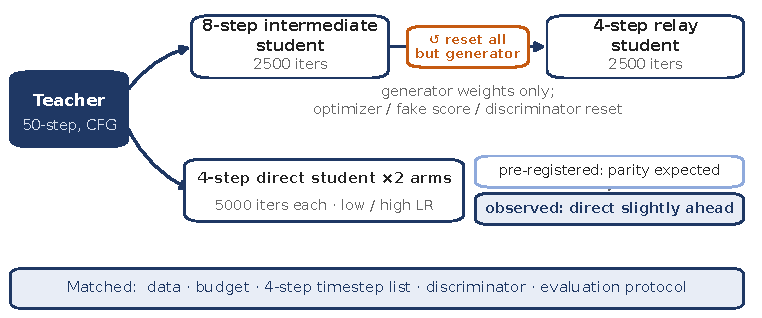
\includegraphics[width=\linewidth]{../figures/fig1_relay_design.pdf}
  \caption{The step-count relay and the matched controlled design. The 50-step teacher forks into a relay path through an 8-step intermediate student (only generator weights cross the handoff; optimizer, fake score, and discriminator re-initialize) and two direct-distillation arms; data, budget, timestep list, discriminator, and evaluation protocol are matched, and the comparison was preregistered with a neutral hypothesis.}
  \label{fig:relay-design}
\end{figure}

\subsection{System Setup}\label{sec:overview-setup}

All training in this report runs on NVIDIA FastGen (NVlabs, Apache-2.0) \cite{fastgen}, reusing its native DMD2 implementation and its official Wan2.1-T2V-1.3B configuration unchanged; Table~\ref{tab:config} lists the full configuration.

\begin{table}[htbp]
  \centering
  \footnotesize
  \setlength{\tabcolsep}{4pt}
  \begin{tabular}{lp{9.5cm}}
    \toprule
    Setting & Value \\
    \midrule
    \multicolumn{2}{l}{\textbf{Inherited from upstream (stock values)}} \\
    \midrule
    Teacher guidance & CFG scale 5 \\
    Adversarial weight (generator side) & 0.03 \\
    Discriminator $(t, \varepsilon)$ pairing & shared draw for real and fake (stock) \\
    Discriminator & trainable multiscale MLP heads on frozen teacher layers 15/22/29 \\
    Update ratio & 5 fake-score updates per generator update \\
    4-step timestep list & $[0.999, 0.937, 0.833, 0.624, 0.0]$ \\
    \midrule
    \multicolumn{2}{l}{\textbf{This project (schedule layer)}} \\
    \midrule
    Stage 1 & 8-step student: LR 1e-5, global batch 12, 2500 iterations \\
    Stage 2 & 4-step student: LR 5e-6, global batch 16, 2500 iterations, generator-only inheritance \\
    Training data & OpenVid-1M (webdataset) \\
    Hardware & 8$\times$ RTX 5090, 32 GB each (shared node) \\
    \bottomrule
  \end{tabular}
  \caption{Training configuration. Upper block: single-stage settings inherited unchanged from the upstream FastGen Wan2.1 configuration. Lower block: this project's schedule layer.}
  \label{tab:config}
\end{table}

The upstream repository provides only one-stage 50$\to$4 and 50$\to$2 configurations. On top of that stack, this project's contribution is confined to the training-schedule layer — the 50$\to$8$\to$4 step-count relay, in which the 4-step stage inherits only the generator weights of the selected 8-step checkpoint and re-initializes optimizer, fake score, and discriminator — together with the choice of training data, OpenVid-1M \cite{openvid}, which the upstream recipe leaves open, and the audit and evaluation protocol of this report. No improvement to the upstream implementation is claimed; every single-stage hyperparameter is upstream's design.

Evaluation is built around VBench \cite{vbench} together with seed-controlled diversity and optical-flow motion measures; Section~\ref{sec:protocol} specifies each instrument and the reason it is there.

%%MD04
\section{Distillation Training and Acceleration}\label{sec:training}

This chapter describes what was trained and what it achieved: a two-stage schedule from 50 steps down to 4, a June 2026 campaign whose failures produced two working rules, and a $\approx$25$\times$ wall-clock speedup.

\subsection{The Step-Count Relay Recipe}\label{sec:training-recipe}

The DMD2 objective \cite{dmd1,dmd2} and every single-stage hyperparameter come unchanged from NVIDIA FastGen's public configuration for Wan2.1-T2V-1.3B \cite{fastgen,wan21} (Section~\ref{sec:overview}); what this project adds is the schedule layer.

The upstream repository distills the 50-step teacher to 4 or 2 steps in one stage. The present work instead trains through an intermediate step count — a \textbf{step-count relay}: a staged schedule that distills 50$\to$8$\to$4, re-initializing everything but the generator between stages (Figure~\ref{fig:relay-design}). Stage one trains an 8-step intermediate student from the teacher, on a nine-anchor timestep list interpolated densely toward the high-noise end. Stage two trains the 4-step student on the unchanged upstream anchors ($t = 0.999$, 0.937, 0.833, 0.624, terminating at 0), inheriting exactly one thing from stage one: the generator weights of its selected checkpoint (the final one, chosen by inspection at the time; see Section~\ref{sec:discussion-limitations}). The optimizer state, the fake score network (DMD2's trainable estimate of the student's own distribution), and the discriminator all restart from scratch. Throughout both stages the discriminator is the upstream design, trainable multiscale MLP heads reading intermediate-layer features of the frozen teacher backbone; the training data is OpenVid-1M \cite{openvid}. Checkpoints are archived every 500 iterations, a habit that becomes important in Section~\ref{sec:protocol}.

The intuition behind the relay is simple: two milder compressions may be easier to learn than one jump from 50 steps to 4. The protocol itself is not new; image-domain distillation has relayed through intermediate step counts before \cite{sdxllightning,hypersd}. Whether the relay is actually worth its extra stage is left open in this chapter; Section~\ref{sec:experiments} settles it under matched-budget, single-variable conditions.

\subsection{Training History and Engineering Lessons}\label{sec:training-history}

The recipe above came out of seven training runs in June 2026, and the most durable products of that month are two rules.

The campaign opened with a direct 50$\to$4 run at a conservative learning rate (1.25e-6, global batch size 8, 6,000 iterations) — the weak-recipe direct run — whose job was to prove that training, checkpointing, and inference close end to end. It did, and its timing sweep also produced the $\approx$25$\times$ speedup reported in Section~\ref{sec:training-acceleration}.

The 8-step intermediate stage absorbed most of the month's failures. One early attempt came out visibly blurry and survives only as a note, for reasons given below. Another swapped in a uniform timestep list and produced a textbook mode collapse; that failed run later became a useful positive control, and Section~\ref{sec:protocol-control} returns to it. The stage worked only after the learning rate went back up to the upstream default of 1e-5 (global batch size 12, 2,500 iterations, roughly 500 generator updates under the upstream one-update-in-five ratio): by visual inspection, the 8-step student was judged good enough to relay from. Its final checkpoint seeded two successive rounds of the 4-step stage. The first broke down visibly late in training; the second — learning rate 5e-6, global batch size 16, 8 GPUs, 2,500 iterations — became the relay student that the rest of this report examines.

Two lessons became methodology. First, attribution: between those two rounds, three factors changed at once — learning rate (1e-5 to 5e-6), global batch size (12 to 16), GPU count (6 to 8). The second round looked better, but the improvement cannot be attributed to any one of the three. Every experiment thereafter changes exactly one major factor; that rule shapes the controlled designs of Section~\ref{sec:experiments}. Second, evidence: the run directory of the blurry 8-step attempt disappeared from the server before it was ever quantitatively evaluated, so ``it was blurry'' remains an unverified anecdote. Every run since is bound to a triple: one config, one run directory, one results note, with the config stored inside the run directory as the sole hyperparameter ground truth.

By the end of June, visual inspection suggested that the relay student improved steadily the longer it trained. Section~\ref{sec:protocol} re-measures that impression, and it does not hold.

\subsection{Acceleration Results}\label{sec:training-acceleration}

The speedup is measured as per-video wall-clock time on the same GPU model (RTX 5090), averaged over the same ten prompts, timed per single 480p, 81-frame video. The teacher samples 50 denoising steps with classifier-free guidance (scale 5), which doubles each step into two forward passes — roughly 100 network function evaluations (NFE) per video — and averages 165.24 s. The 4-step student drops guidance entirely, spending 4 NFE and 6.59–6.66 s per video across the full checkpoint sweep: a $\approx$25$\times$ speedup (24.83–25.07$\times$ depending on checkpoint), first measured on 2026-06-15 and re-verified on 2026-07-26 against the run's raw per-video timing records.

The number matches the arithmetic exactly. A 100:4 ratio of network evaluations predicts 25$\times$, and the measured wall-clock ratio lands on it: the entire latency gain comes from removing steps and guidance, and the student adds no inference overhead of its own. The timing is also a property of the inference path rather than of any training recipe. The band was measured on the weak-recipe run's checkpoint sweep, and every other 4-step student in this report samples through an identical guidance-free path, so per-video cost does not depend on how the student was trained.

Speed is therefore the easy half of the result. Any 4-step student of this backbone runs $\approx$25$\times$ faster; the question that separates one such student from another, and occupies every remaining section, is what those four steps can still generate.

%%MD05
\section{Evaluation Protocol}\label{sec:protocol}

Every conclusion in Section~\ref{sec:experiments} is a comparison between numbers, so this chapter answers the question a skeptical reader will ask first: why not simply watch the videos? For the first month, quality was judged by visual inspection. This failed in a measurable way.

\subsection{Why Subjective Checkpoint Selection Fails}\label{sec:protocol-subjective}

Through June 2026, every quality judgment in this project was made by eye, on a handful of prompts in-domain with the training data. In July 2026, all stored checkpoints — twelve models accumulated across the project's training lines — were scored in one pass under the quantitative protocol of Section~\ref{sec:protocol-audit}. On both lines where the subjective pick could be tested, it was overturned, in opposite directions.

On the relay line, inspection had picked the final checkpoint, under the recorded impression that quality improved steadily with training. The scores disagree: aesthetic quality is highest at the very first checkpoint and slides across the sweep, from 0.5768 at iteration 500 to 0.5379 at the chosen iteration 2500 (150 standard prompts, single seed), and the quantitative optimum sits at iterations 500–1000. The subjective pick was too late. On the weak-recipe direct-distillation line, inspection had picked iteration 1000; under the same protocol, the checkpoint 500 iterations later outscores it on five of the six dimensions — aesthetic quality 0.5357 against 0.5103, imaging quality 0.6847 against 0.6341, among others. The subjective pick was too early.

One reversal could be chance. Two reversals in opposite directions indicate a property of the method: subjective checkpoint selection is systematically unreliable here. The two records can be reconciled: during training, the viewer watched those in-domain prompts for one thing, the repair of physical plausibility, which the six benchmark dimensions on the standard prompt set do not measure. Both records can be true at once; only one supports comparisons.

The replacement is mechanical. Every run saves a checkpoint every 500 iterations; every checkpoint is scored under the identical protocol; the checkpoint with the best joint reading of the six dimensions is selected (full-sweep checkpoint selection; when two checkpoints split the dimensions, both are carried forward), and only the selected checkpoints are re-scored under three seeds, which supply the numbers a claim may cite. Selection and estimation are thereby separated. Figure~\ref{fig:sweep-curves} plots aesthetic quality against training iteration for every checkpoint of the relay student and its matched direct-distillation counterpart (defined in Section~\ref{sec:exp-relay}; the relay spends its first 2500 iterations at 8 steps). Both curves share a feature: quality peaks within the first 500–1000 iterations and then trends downward. Why longer training makes a student worse is answered in Section~\ref{sec:exp-audit}.

\begin{figure}[htbp]
  \centering
  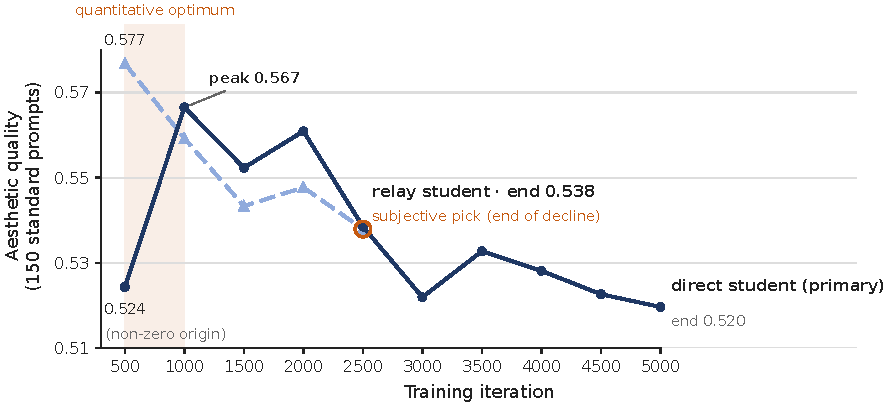
\includegraphics[width=\linewidth]{../figures/fig4_sweep_curves.pdf}
  \caption{Aesthetic quality (150 standard prompts, seed 0) across the full checkpoint sweeps of the relay student (5 checkpoints) and the direct student (10 checkpoints). The direct-arm trajectory is a single-seed sweep quoted as pattern only. Quality peaks within iterations 500--1000 (shaded); the subjectively picked relay endpoint sits at the end of a decline. Non-zero origin.}
  \label{fig:sweep-curves}
\end{figure}

\subsection{The Four-Component Audit Protocol}\label{sec:protocol-audit}

The protocol that replaced visual inspection has four components. Each is there because a simpler instrument failed or would have misled.

\textbf{Six quality dimensions on a standard set.} VBench in custom-input mode \cite{vbench} scores subject consistency, background consistency, motion smoothness, dynamic degree, aesthetic quality, and imaging quality on 150 prompts sampled deterministically from the official all-dimension suite. The set is compact enough to score every checkpoint of every run — it is the instrument behind full-sweep selection — with sweeps run at a single seed and selected checkpoints re-scored at three.

\textbf{Dynamic degree on a clean motion set.} One of the six readings cannot be trusted on the standard set: it contains prompts that instruct stillness, so a model that obeys them is scored as unable to move. The teacher reads 0.300 on the 150-prompt set but 0.625 on a 40-prompt motion set — the same model and metric; the gap is the confound. Dynamic degree is therefore quoted only on the motion set: 40 motion-oriented prompts, 20 sampled at uniform stride from the official human-action list and 20 from the standard suite, retained only if they carry an explicit motion cue and none of a static-phrase blacklist. Standard-set readings are reported only as footnotes.

\textbf{Cross-seed diversity.} All six dimensions score each video in isolation; none asks whether different noise draws yield different videos. Diversity is measured as the mean pairwise LPIPS \cite{lpips} (AlexNet backbone) among eight generations per prompt — eight seeds on a fixed set of 40 prompts; higher is more diverse. Section~\ref{sec:experiments} relies on this component most: it measures what turns out to be the principal axis of degradation.

\textbf{Continuous motion amplitude.} Binary dynamic degree saturates for capable students — every student measured on the motion set reads 0.75–1.0, at or above the teacher's 0.625 — so it cannot rank models that all move. Motion amplitude is therefore measured as RAFT optical flow \cite{raft} in pixels per frame on the same 40 motion prompts, median as the primary reading with the mean alongside, since the distribution is heavy-tailed (teacher: median 2.75, mean 5.16, single seed). Flow readings need care: per-model medians vary by up to a factor of six across seeds, and one seed produced uniformly low readings from all three models under audit (teacher 0.86, the direct and relay students 0.46 and 1.27 pixels per frame). Part of a video's motion level comes from the initial noise rather than the model. Cross-arm flow comparisons are therefore reported as same-direction counts over shared seeds, and no single-seed absolute percentage is quoted on its own.

For headline tables the report switches to the full VBench standard protocol — the official 946 prompts at 5 seeds each — covering 12 of the 16 dimensions; the missing four depend on an external object-detection stack that was not installed, and every such table says so. Two rules hold everywhere: numbers never travel across prompt domains, and training-health signals such as loss curves are never quality evidence. Prompt lists, checksums, and sampling scripts for all sets are catalogued in Appendix~\ref{sec:app-protocol} under the codenames q150, dm40, d40, and vb946.

\subsection{Positive Control and Blind Spots}\label{sec:protocol-control}

A protocol should also be shown to catch a broken model. This one was tested by accident. One June recipe attempt — an 8-step student trained with a uniform timestep schedule, anchors spread evenly instead of concentrated at high noise — failed, and its scores are why the protocol's joint-reading rule exists. In the twelve-model scan (150 standard prompts, single seed), that model is the best of the table on both consistency dimensions (subject consistency 0.9745 and background consistency 0.9791, above the teacher's 0.9661 and 0.9642) and the worst on imaging quality (0.2555), aesthetic quality (0.3181), and cross-seed diversity (0.4617; 40 prompts $\times$ 8 seeds). Its dynamic degree on the same standard set, 0.1867, sits below even the teacher's confounded 0.300. The most consistent model in the project is a collapsed one. It produces near-static frames and near-duplicate seeds, yet it earns the highest consistency scores in the table.

Any reading of consistency alone, or of an aggregate that weights consistency heavily, would select this model as the winner. Hence the rule enforced throughout Section~\ref{sec:experiments}: consistency-type dimensions are interpreted only alongside dynamic degree and cross-seed diversity, and a student scoring at or above the teacher on consistency is read as reduced frame-to-frame change rather than as a quality gain. The failure mode itself is not new — a uniform timestep schedule inducing a collapse that aggregate benchmark scores miss has been reported before \cite{tmd}, and no priority is claimed; what this reproduction adds is a live positive control inside the project's own tables. What the positive control cannot test is the same blind spot at benchmark scale. Section~\ref{sec:exp-vbench} returns to it there, where an official composite score misses it in the same way.

%%MD06
\section{Experiments: Diagnosis and Attribution}\label{sec:experiments}

Section~\ref{sec:training} cut the teacher's fifty denoising steps to four, and the resulting videos look intact at first viewing. This section asks what first viewing cannot settle: what exactly was lost, and which part of the training system is responsible. The answers arrive in order: a diagnosis (Section~\ref{sec:exp-diversity}), controlled comparisons (Sections~\ref{sec:exp-relay} and~\ref{sec:exp-audit}), an attribution (Section~\ref{sec:exp-attribution}), and an external benchmark check (Section~\ref{sec:exp-vbench}).

\subsection{Main Finding: Diversity Collapse, Not Motion Collapse}\label{sec:exp-diversity}

Prior reports raise a specific concern: when video diffusion models are distilled to a few steps, motion degrades first and the missing dynamics are the price of speed \cite{dataforcing,phaseddmd}. The quantitative result is the opposite. On the 40 motion-oriented prompts, every evaluated student — weak and matched recipes, relay and direct paths, the 8-step intermediate alike — scores a dynamic degree of 0.750–1.000 against the teacher's 0.625. By this measure the students move more than the teacher. The extra movement is also not jitter: motion smoothness holds at 0.970–0.987 across the measured students, barely below the teacher's 0.985. One boundary is deliberate: those motion-loss reports come from other settings (an image-to-video model in one case, a larger Wan variant in the other), so the claim here is only that the motion collapse was not reproduced in this setting, without refuting those reports.

What collapsed is something no single video reveals: variety across random seeds. Cross-seed diversity — mean pairwise LPIPS \cite{lpips} over 8 seeds per prompt, higher meaning more diverse — falls from the teacher's 0.732 to 0.586–0.649 across every 4-step student and the 8-step intermediate (40 prompts $\times$ 8 seeds; the intermediate's own readings: dynamic degree 0.950, diversity 0.5949). Figure~\ref{fig:dd-diversity} puts the two axes side by side: dynamic degree up, diversity down. Figure~\ref{fig:seed-grid} shows what the number means. Given one prompt and eight seeds, the teacher returns eight different videos, with different compositions, camera placements, and palettes; the students return eight variations of one template. Each clip is individually presentable; that is the picture behind 0.732 versus 0.59–0.64. Because every clip is fine on its own, no metric that scores videos one at a time can see the loss; it appears only under repeated sampling of the same prompt, which the protocol of Section~\ref{sec:protocol} does.

\begin{figure}[!tb]
  \centering
  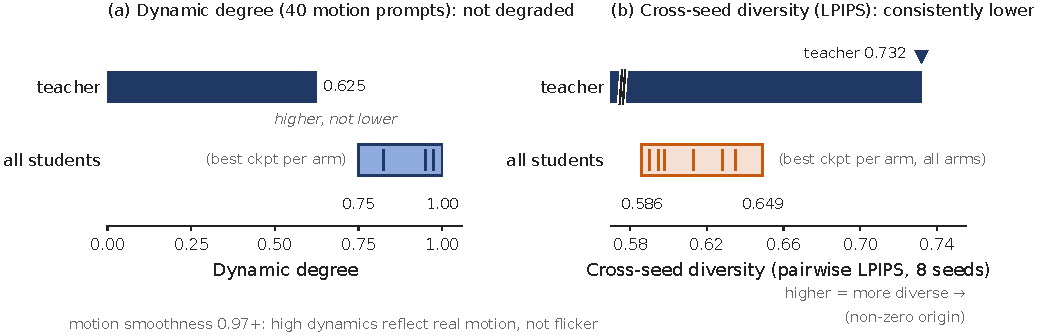
\includegraphics[width=\linewidth]{../figures/fig3_dd_diversity_panels.pdf}
  \caption{(a) Dynamic degree on the 40 motion-oriented prompts: the teacher against the selected checkpoint of every arm — higher, not lower. Motion smoothness stays at 0.970--0.987, so high dynamics reflect real motion rather than flicker. (b) Cross-seed diversity (mean pairwise LPIPS, 40 prompts $\times$ 8 seeds; non-zero origin): the teacher's 0.732 against 0.586--0.649 across all arms' selected checkpoints — the principal degradation axis.}
  \label{fig:dd-diversity}
\end{figure}

\begin{figure}[!tb]
  \centering
  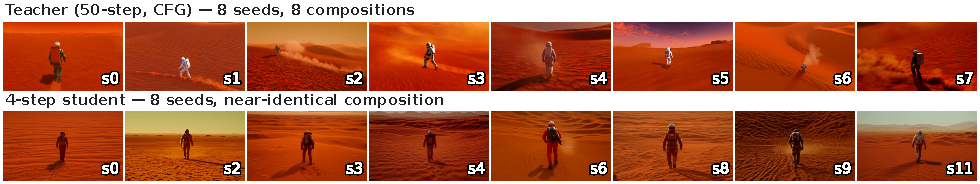
\includegraphics[width=\linewidth]{../figures/fig6_seed_grid.pdf}
  \caption{One prompt, eight random seeds (40th frame of each video, seed IDs as labeled). Top: the 50-step teacher returns eight visibly different compositions. Bottom: the 4-step direct student returns near-identical framings — the visual form of the diversity numbers in Figure~\ref{fig:dd-diversity}. The two panels use their respective demo seed pools; the quantitative diversity protocol uses its own fixed 8-seed set, so this grid illustrates rather than constitutes the measurement.}
  \label{fig:seed-grid}
\end{figure}

The drop appears in the weak-recipe pilot and the matched recipes, in relay-trained and directly trained students, with the adversarial branch on and off, in the same direction every time; it is the most-replicated observation of the project. The rest of this section searches for its source: one controlled family swaps the training path (Section~\ref{sec:exp-relay}), the other operates on the discriminator (Section~\ref{sec:exp-audit}).

\subsection{Controlled Comparison: Relay versus Direct Distillation}\label{sec:exp-relay}

The step-count relay was this project's original design (Section~\ref{sec:training}), so it received the most scrutiny. The comparison against one-stage direct distillation (50$\to$4) was run as a controlled experiment, with the hypothesis registered in advance while the matched arms were still training. The registered hypothesis was neutral (the two paths should be comparable), since a weak-recipe direct student had already matched the relay on most dimensions; the selection criteria — the six quality dimensions read jointly with cross-seed diversity — were fixed at registration. To the best of the authors' knowledge, this is the first controlled relay-versus-direct comparison on this base model; direct few-step distillation is established practice on this backbone \cite{fastwan,codmd} but had not been weighed against a relay under matched conditions.

The two paths were matched on everything except the schedule (Figure~\ref{fig:relay-design}), with checkpoints every 500 iterations and full-sweep selection in every arm. The relay spent 2500 iterations at 8 steps and 2500 at 4 steps; each direct arm received the same 5000-iteration budget. Because the relay's two stages use different recipes, two direct arms bracket it (Table~\ref{tab:setup}), so an untuned direct baseline cannot explain the outcome.

\begin{table}[htbp]
  \centering
  \begin{tabular}{lll}
    \toprule
    Arm & Recipe (LR / global batch) & Schedule \\
    \midrule
    Relay & 1e-5/12 $\to$ 5e-6/16 & 8-step 2500 + 4-step 2500 \\
    Direct (primary) & 5e-6/16 & 4-step 5000 \\
    Direct B & 1e-5/12 (upstream stock) & 4-step 5000 \\
    \bottomrule
  \end{tabular}
  \caption{The three arms of the controlled comparison; total budget 5000 iterations each, all other factors matched.}
  \label{tab:setup}
\end{table}

Table~\ref{tab:g2} reports the verdicts. On quality the arms are close to a tie, with a slight edge to the direct path. Aesthetic differences sit inside the checkpoint jitter band (direct 0.567 against relay 0.577/0.559), with the teacher's 0.590 above all of them. Imaging is the direct student's one measured edge: 0.717 against the relay's sweep-best 0.697, a gap of 0.020 where adjacent-checkpoint jitter runs about 0.005–0.015. That 0.717 is also above the teacher's 0.692 and is read as a sharpness bias rather than a genuine quality gain, the same kind of static bias as the consistency rule of Section~\ref{sec:protocol-control}. A three-seed re-scoring of the selected checkpoints kept every verdict — aesthetic 0.591 [0.580, 0.603] (mean [seed minimum, seed maximum]) for the teacher against 0.563 [0.543, 0.580] direct and 0.570 [0.559, 0.590] relay (iteration 1000) — and softened one: the imaging edge became ``not lower than the relay'' rather than ``above it.'' On the diversity axis of Section~\ref{sec:exp-diversity}, the result is one-sided: both direct arms retain more cross-seed diversity than the relay (0.635 and 0.628 versus 0.598–0.613), with two independently trained runs agreeing in direction (gaps 0.015–0.037). The relay makes the main degradation worse. One number runs the other way: the direct student is the least mobile, dynamic degree 0.750 against 0.825–1.000 for the relay and 0.975 for direct student B, above the teacher's 0.625 but the lowest of the students. The deliverable model of this project is therefore the direct student at iteration 1000: with quality tied inside the jitter band, the preregistered protocol reads the diversity axis, where both direct arms lead.

\begin{table}[htbp]
  \centering
  \footnotesize
  \setlength{\tabcolsep}{4pt}
  \begin{tabular}{lrrrr}
    \toprule
    Model (codename), checkpoint & Aesthetic & Imaging & Dynamic degree & Diversity \\
    \midrule
    Teacher, 50-step, CFG 5 & 0.590 & 0.692 & 0.625 & 0.732 \\
    Direct student (E1a), iter 1000 & 0.567 & 0.717 & 0.750 & 0.635 \\
    Relay student (W7), iter 500 & 0.577 & 0.694 & 0.825 & 0.598 \\
    Relay student (W7), iter 1000 & 0.559 & 0.697 & 1.000 & 0.613 \\
    Direct student B (E1b), iter 500 & 0.532 & 0.695 & 0.975 & 0.628 \\
    Weak-recipe direct student (W1), iter 1000 — reference & 0.510 & 0.634 & 0.950 & 0.649 \\
    \bottomrule
  \end{tabular}
  \caption{Relay versus direct distillation at the selected checkpoints; the relay's sweep splits its leading dimensions across iterations 500 and 1000, so both are shown, and the deliverable model is the direct student at iteration 1000. Aesthetic and imaging: 150 standard prompts, seed 0. Dynamic degree: 40 motion-oriented prompts. Cross-seed diversity: mean pairwise LPIPS, 40 prompts $\times$ 8 seeds.}
  \label{tab:g2}
\end{table}

The relay's one consistent real difference is motion amplitude: median optical flow \cite{raft} on the 40 motion prompts, paired per seed across four seeds (Table~\ref{tab:flowdir}).

\begin{table}[htbp]
  \centering
  \begin{tabular}{lrr}
    \toprule
    Comparison & Same direction & By 4-seed means \\
    \midrule
    Relay vs direct & 4 of 4 seeds & 3.36 vs 1.81 ($\approx$1.9$\times$) \\
    Relay vs teacher & 4 of 4 seeds & +64\% \\
    Direct vs teacher & 3 of 4 below & $-$12\% \\
    \bottomrule
  \end{tabular}
  \caption{Motion amplitude, paired per seed (median RAFT flow, 40 motion prompts; per-seed values in Appendix~\ref{sec:app-flow}).}
  \label{tab:flowdir}
\end{table}

Whether this counts for or against the relay depends on the criterion — fidelity to the teacher's motion distribution favors the direct student, maximal motion favors the relay — and this report does not take a side. The binary dynamic degree, saturated at 0.75–1.0 for both arms, hides this 1.9$\times$ difference; the continuous flow measure exists in the protocol for this reason (Section~\ref{sec:protocol}).

Figure~\ref{fig:sweep-curves} plots quality against training iteration for the full sweeps. Both adversarially trained arms peak early and then decline: the relay's aesthetic slides from 0.577 at iteration 500 to 0.538 at 2500, and the direct student's from a 0.567 peak at iteration 1000 to 0.520 at 5000 (not strictly monotonic). Training longer made both students worse. The discriminator audit was built to identify which component does that and which maintains the relay's extra motion.

\subsection{Discriminator Audit: Three-Arm Ablation}\label{sec:exp-audit}

DMD2 training carries an adversarial branch: trainable multiscale heads on frozen teacher features, whose gradient reaches the generator at weight 0.03 (Section~\ref{sec:training}). The upstream configuration fixes two conventions \cite{fastgen}: the weight itself, and the shared-$(t, \varepsilon)$ convention, under which the discriminator sees its real and fake inputs corrupted with the same timestep and noise draw. The audit ran two single-variable ablations on the relay recipe, each changing exactly one configuration field: the GAN-off arm sets the adversarial weight 0.03 $\to$ 0, and the independent-pairing arm switches shared-$(t, \varepsilon)$ to independent draws with the weight untouched. Everything else — initialization from the same 8-step checkpoint, learning rate, batch size, the 2500-iteration schedule, the protocol — is identical, verified against the run configurations; the GAN-off checkpoint stores no discriminator weights, consistent with the switch. Table~\ref{tab:threearm} (Appendix~\ref{sec:app-threearm}) lists all fifteen checkpoints; Figure~\ref{fig:gan-bifurcation} draws the three trajectories, which separate within the first thousand iterations.

\begin{figure}[htbp]
  \centering
  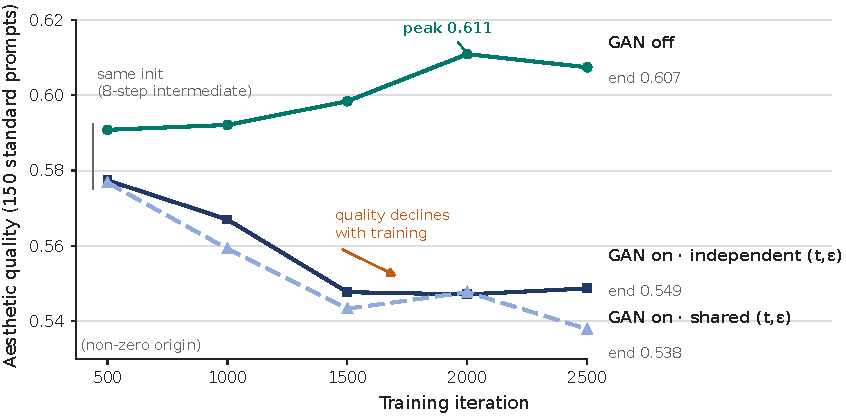
\includegraphics[width=\linewidth]{../figures/fig2_gan_bifurcation.pdf}
  \caption{Aesthetic quality (150 standard prompts, seed 0) against training iteration for the three discriminator-audit arms, all initialized from the same 8-step intermediate checkpoint. With the adversarial branch off, quality climbs across the sweep; both GAN-on arms decline in parallel. Non-zero origin.}
  \label{fig:gan-bifurcation}
\end{figure}

\textbf{The decline follows the adversarial branch.} With the GAN off, the early-peak-then-decline pattern of Section~\ref{sec:exp-relay} reverses rather than merely weakens. Aesthetic climbs from 0.591 to a 0.611 peak at iteration 2000 and imaging rises monotonically 0.701 $\to$ 0.723 (150 standard prompts, seed 0), while both GAN-on arms decay in parallel (0.577 $\to$ 0.538 shared pairing; 0.577 $\to$ 0.549 independent). Re-scored with three seeds at the selected checkpoints (GAN-off at iteration 2000, independent-pairing at 500), the GAN-off arm leads in 3 of 3 seeds on both aesthetic (+0.02–0.03 per seed; means 0.613 [0.600, 0.626] versus 0.587 [0.576, 0.607]) and imaging (+0.01–0.03; 0.723 [0.721, 0.725] versus 0.701 [0.690, 0.714]): consistent in direction, slightly beyond the seed band in magnitude, with the band edges nearly touching. The adversarial branch is thereby a candidate mechanism for the decline — candidate, because the evidence covers a single GAN weight (0.03) on the relay path only, and the GAN-off run's behavior past iteration 2500 was not measured. The GAN-on direct arm shows a matching trajectory in Section~\ref{sec:exp-relay} (peak at 1000, drift to 0.520 by 5000), but this is supporting pattern only: without the ablation, overtraining cannot be excluded there. The GAN-off arm's 0.613 aesthetic against the teacher's 0.590 is higher on static-quality metrics only; it moves at teacher level, and its diversity gap remains (below).

\textbf{Motion amplitude also follows the adversarial branch, but only from a relay start.} (Sweep flow values in this paragraph are seed-0 single points; only directions and trends are quoted.) The GAN-off arm, initialized from the same 8-step student, spends its entire sweep at teacher-level motion (median flow 2.14–2.74 versus the teacher's 2.75). The independent-pairing arm, GAN on, climbs 2.40 $\to$ 4.71, starting below its own 8-step initialization source (3.84) and rebuilding past the relay reference's 4.44. Motion therefore decays at the handoff and the adversarial signal rebuilds it. However, the direct student trains with the same weight and averages 1.81 across four seeds, not above the teacher. Within the tested recipe, elevated motion is therefore an interaction: relay initialization provides the high-motion starting point, and the adversarial signal maintains it. The recipe's independent contribution was not measured under controlled conditions.

\textbf{The shared pairing convention does nothing detectable.} Shared-$(t, \varepsilon)$ corruption is the upstream stock value and is implicit at the notation level in published formulations \cite{aad1}; to the best of the authors' knowledge, neither the surveyed literature nor the twelve public implementations examined had tested it in isolation before this audit. Under the first controlled test, no effect was detected at the $\sim$0.01 resolution of this setup: across all five checkpoint pairs the aesthetic difference never exceeds 0.011 (0.577/0.577, 0.559/0.567, 0.543/0.548, 0.548/0.547, 0.538/0.549), and the quality, diversity, and motion trajectories share the same shape.

An offline probe adds mechanistic background. A linear classifier on the discriminator's own feature path separates real from generated clips perfectly at every layer for low and middle noise levels (AUC 1.0 at $t \le 0.937$, saturated at $n = 64$ per side) and near-randomly at the highest level (0.28–0.52 at $t = 0.999$): the discriminator's usable signal concentrates at low noise, leaving little room for a pairing convention to matter at the top of the range. As a control, the teacher's 50-step generations are just as separable from real data, so separability reflects the generated-versus-real domain gap rather than distillation damage; the probe is recorded as an observational note only. A planned fourth arm (an R1 regularizer on the discriminator, calibrated to a suggested weight of 0.75) hit a deterministic out-of-memory on the 32 GB cards and is recorded as untested; its calibration is archived for reproduction on 80 GB hardware.

One result is common to all three arms: across all fifteen checkpoints, cross-seed diversity sits in 0.586–0.613. The GAN switch moved quality and motion; the pairing switch moved nothing; neither touched the collapse of Section~\ref{sec:exp-diversity}.

\subsection{Attribution: The Collapse Survives Every Tested Component}\label{sec:exp-attribution}

The controlled results combine into an exclusion argument (Figure~\ref{fig:attribution}). Swapping the training path leaves direct students at 0.628–0.635 cross-seed diversity and relay checkpoints at 0.598–0.613, collapsed either way and deeper on the relay, against the teacher's 0.732 (40 prompts $\times$ 8 seeds throughout). Removing the adversarial branch gives 0.586–0.604; changing the discriminator's pairing convention gives 0.590–0.612. Every altered system reproduces the same loss at the same magnitude; the tested components modulate its depth at most, and none creates or removes it. Within the components this project could isolate, the collapse is attributable to the distribution-matching distillation itself — the one element every arm retains — not to its adversarial or scheduling attachments. The consistency-model line has criticized distribution-matching objectives on exactly this ground \cite{rcm}; that criticism here gains a measured, component-controlled instance on a public base model.

\begin{figure}[htbp]
  \centering
  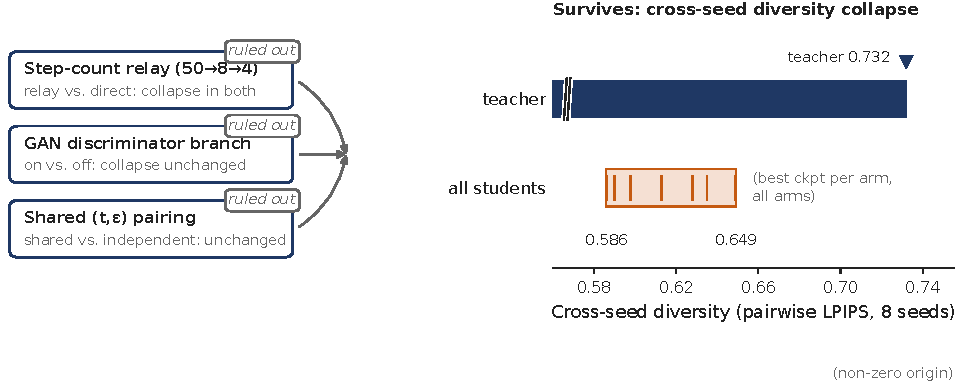
\includegraphics[width=\linewidth]{../figures/fig5_attribution.pdf}
  \caption{Attribution by controlled exclusion: swapping the training path, removing the adversarial branch, and changing the pairing convention each leave the cross-seed diversity collapse in place (teacher 0.732; all students 0.586--0.649 at their selected checkpoints; non-zero origin).}
  \label{fig:attribution}
\end{figure}

The exclusion list is finite: the data composition, the folding of classifier-free guidance into the teacher, other adversarial weights, and score-matching variants remain untested, and any of them could yet move the number (Section~\ref{sec:discussion} returns to these). What this work delivers is therefore not a remedy but a problem definition with the measurement attached: a specific quantity, cross-seed diversity falling from 0.732 to 0.59–0.64, stable under every intervention tested here; no impossibility claim is made either.

\subsection{External Benchmark: VBench Across Twelve Dimensions}\label{sec:exp-vbench}

Would any of this be visible from the outside? Scoring the four main models on VBench \cite{vbench}, across 12 of its 16 dimensions on the standard suite, returns a split picture rather than a ranking (Table~\ref{tab:vbench}): no model dominates, and the twelve per-dimension best scores are split across three of the four students, several by margins under a thousandth. The direct student takes the temporal-stability rows (motion smoothness 0.9812, temporal flickering 0.9894); the relay student takes motion and action semantics (dynamic degree 0.9111, human action 0.794, temporal style 0.2305); the GAN-off arm takes the remaining seven, static quality (aesthetic 0.6482, imaging 0.6924) plus the consistency, scene, and appearance rows. Direct student B leads no row and sits mid-field, its profile tilted the relay's way (dynamic degree 0.8806, aesthetic 0.5802). Each student leads on a different axis, and the diversity upper bound stays with the teacher: the picture of Section~\ref{sec:exp-diversity} at benchmark scale. The teacher itself is absent from these tables: scoring it under the 946-prompt protocol was not affordable within the project window, so teacher references in this report come from the audit protocol of Section~\ref{sec:protocol}.

\begin{table}[htbp]
  \centering
  \footnotesize
  \setlength{\tabcolsep}{4pt}
  \begin{tabular}{lrrrr}
    \toprule
    Dimension & Direct student & Relay student & Direct student B & GAN-off arm \\
              & (E1a) @1000 & (W7) @1000 & (E1b) @500 & (E2a) @2000 \\
    \midrule
    subject\_consistency & 0.9727 & 0.9693 & 0.9673 & 0.9753 \\
    background\_consistency & 0.9579 & 0.9508 & 0.9416 & 0.9581 \\
    motion\_smoothness & 0.9812 & 0.9727 & 0.9747 & 0.9786 \\
    dynamic\_degree & 0.5806 & 0.9111 & 0.8806 & 0.8000 \\
    aesthetic\_quality & 0.5967 & 0.6087 & 0.5802 & 0.6482 \\
    imaging\_quality & 0.6687 & 0.6687 & 0.6614 & 0.6924 \\
    temporal\_flickering & 0.9894 & 0.9796 & 0.9810 & 0.9878 \\
    human\_action & 0.690 & 0.794 & 0.716 & 0.776 \\
    scene & 0.2173 & 0.2922 & 0.2225 & 0.2974 \\
    appearance\_style & 0.1990 & 0.1982 & 0.2003 & 0.2010 \\
    temporal\_style & 0.2214 & 0.2305 & 0.2260 & 0.2283 \\
    overall\_consistency & 0.2240 & 0.2386 & 0.2298 & 0.2391 \\
    \bottomrule
  \end{tabular}
  \caption{VBench, standard suite (946 prompts $\times$ 5 samples), the 12 of 16 dimensions runnable here. The GAN-off column is the audit arm, added for completeness at a single checkpoint; the deliverable model remains the one selected under the preregistered protocol. Dynamic degree on this suite is not comparable with the motion-prompt dynamic degree quoted elsewhere in this report.}
  \label{tab:vbench}
\end{table}

The official composite is more instructive (Table~\ref{tab:qs}). Folding the seven quality dimensions into VBench's Quality Score places the GAN-off arm first at 85.50, the relay student at 84.47, direct student B at 83.62, and the preregistered primary model last at 82.80, pulled down by its dynamic degree (0.5806, entering at half weight). The score has no diversity term, so the arm with the lowest diversity band among the four benchmarked models (0.586–0.604) ranks first, and the main degradation axis of this report is structurally invisible to the score. This repeats at benchmark scale the blind spot the positive control exposed in Section~\ref{sec:protocol}: no VBench dimension measures variety across seeds, which is why the seed-controlled protocol exists.

\begin{table}[htbp]
  \centering
  \begin{tabular}{lr}
    \toprule
    Model (codename), checkpoint & Quality Score \\
    \midrule
    GAN-off arm (E2a) @2000 & 85.50 \\
    Relay student (W7) @1000 & 84.47 \\
    Direct student B (E1b) @500 & 83.62 \\
    Direct student (E1a) @1000 — preregistered selection & 82.80 \\
    \bottomrule
  \end{tabular}
  \caption{VBench Quality Score, synthesized from the seven quality dimensions with the official per-dimension min–max normalization and weights (all 1, dynamic degree 0.5; weighted sum divided by 6.5). The composite contains no diversity term.}
  \label{tab:qs}
\end{table}

Three disclosures apply to these tables. Four dimensions that require an external detection model could not be run, so the official Semantic and Total scores cannot be synthesized. The temporal-flickering dimension was scored on a sample set that deviates from the official protocol. The relay student's 84.47 sits one hundredth from a published 84.46 \cite{codmd}: a numeric coincidence between a 7-dimension composite and a 16-dimension total, so no comparison is drawn, and none is valid. Model selection is unaffected: the deliverable remains the direct student chosen under the preregistered protocol of Section~\ref{sec:exp-relay}, despite the composite ranking.

%%MD07
\section{Discussion and Limitations}\label{sec:discussion}

\subsection{Discussion}\label{sec:discussion-discussion}

Section~\ref{sec:experiments} closed with a candidate mechanism and an open problem; this section weighs how much interpretation each carries.

The early quality peak and later decline wherever the adversarial branch is active (Section~\ref{sec:exp-audit}) admit two readings. The decline may be the intrinsic cost of an adversarial objective, with fidelity traded past some point for whatever the discriminator rewards. Or it may be circumstantial: the evidence comes from a single configuration — batch size 16, 2500 iterations, no discriminator regularization, a single adversarial weight of 0.03, the relay path only — and a discriminator trained on such a small budget may simply be unstable, degrading the generator with it. The data cannot distinguish the two. Some observations lean toward systematic pressure rather than failure to converge: the decline is smooth and sustained, training losses never diverge, and the pattern repeats in direction across two independent runs differing only in a convention shown not to matter. No verdict is drawn from these.

An experiment specified but not run here can separate the two readings: the regularized-discriminator arm, calibrated and archived after exceeding the 32 GB memory of the available cards, becomes a deciding experiment on 80 GB-class hardware. If a stabilized discriminator removes the decline, the configuration reading wins; if the decline survives, the intrinsic reading strengthens. A larger-batch control would separate them the same way.

One relay result invites a simpler, less flattering explanation, offered as unquantified interpretation. The relay student's clearest benchmark lead, 0.794 against the direct student's 0.690 on human action (946 prompts $\times$ 5 samples, Section~\ref{sec:exp-vbench}), may reflect motion amplitude more than action understanding: an action scores only when visibly performed, the relay student out-moves the direct student by roughly 1.9$\times$ (per-seed paired optical flow, Section~\ref{sec:exp-relay}), and actions performed with little motion may fail a strict scorer. The impression that the relay student's physics look more natural has no quantitative support and enters no conclusion. The relay path retains one byproduct: the 8-step intermediate student, quantified under the same protocol and deployable wherever eight steps are affordable.

A methodological point follows: widely inherited defaults deserve controlled audits. The shared-pairing convention and the 0.03 weight arrived as stock values, and no surveyed paper or public implementation had tested either in isolation. Audited, they split: for the pairing convention no effect was detected — one setting later practitioners can leave at its default — while the stock weight appears to sit at a working point trading static quality against motion amplitude. Auditing inherited defaults is therefore useful in itself.

The diversity collapse outlasted every audit; why it should attach to the objective itself has a theoretical lead rather than a proof. DMD-family objectives minimize an approximate reverse KL divergence \cite{dmd1,dmd2}, the mode-seeking direction, which in theory narrows the variance of the learned distribution \cite{fdistill}; eight seeds converging toward one template is precisely that narrowing. The fake-score branch is the designed counterweight but must track the student's moving distribution in real time; wherever tracking lags, the narrowing pressure passes through. Criticism of distribution matching on this quality–diversity axis exists \cite{rcm,piflow}, and a data-level regularization route targets the same collapse in few-step video distillation \cite{dataforcing}. Nothing here measures mode-seeking directly; what matches is the direction.

The report stops there deliberately. Section~\ref{sec:exp-attribution} hands over a specification: a named quantity, a measured drop — 0.732 to 0.59–0.64 in mean pairwise LPIPS, 40 prompts $\times$ 8 seeds — and the components ruled out under control. The natural sequel is an intervention study: a diversity-aware term in the training signal, data-level regularization, or first instrumenting how faithfully the fake score tracks the student. None of that is promised here; the problem is now bounded.

\subsection{Limitations}\label{sec:discussion-limitations}

The boundaries of this work:

\begin{itemize}
  \item No human evaluation was run; a planned T2VHE-style study \cite{t2vhe} remains unexecuted, so every conclusion rests on automated metrics.
  \item Four detector-dependent dimensions of the standard benchmark could not be run; the official Semantic and Total composites cannot be synthesized (Section~\ref{sec:exp-vbench}).
  \item The regularized-discriminator arm was never trained (deterministic out-of-memory on the 32 GB cards); its calibration and configuration are archived for reproduction on 80 GB-class hardware.
  \item Every configuration is a single training run, so run-to-run variance is unquantified; same-recipe arms agreeing in direction is the recorded mitigation.
  \item The relay's intermediate checkpoint was chosen by inspection before full-sweep selection became the standard; the relay's ceiling under optimal intermediate selection is unexplored.
  \item The adversarial ablation covers a single weight (0.03), on the relay path only.
  \item One base model, one dataset, one scale: 1.3B parameters at 480p.
  \item The 150-prompt standard quality suite is out-of-domain for the training data.
  \item Checkpoints were archived every 500 iterations; a true peak between archives would be missed.
  \item Sweep quality numbers are largely single-seed (seed 0); only the selected checkpoints were re-scored with three seeds.
  \item Motion amplitude is seed-sensitive; it is reported as per-seed pairs, and single-seed absolutes are not treated as claims.
  \item The audit protocol is ablation-scale by design; its numbers are not directly comparable with full-protocol figures in the literature (the benchmark tables of Section~\ref{sec:exp-vbench} carry their own disclosures).
\end{itemize}

%%MD08
\section{Conclusion}\label{sec:conclusion}

This project distilled Wan2.1-T2V-1.3B from 50 sampling steps to 4, cutting generation from 165.24 to roughly 6.6 seconds per video, a $\approx$25$\times$ speedup that matches the arithmetic of the removed network evaluations. The report's substance is what a seed-controlled audit found behind that number. The audit found no motion collapse: every student's dynamic degree is at or above the teacher's, while motion amplitude differs by arm rather than dropping across the board. The principal degradation is cross-seed diversity, falling from the teacher's 0.732 to 0.59–0.64 in mean pairwise LPIPS over eight seeds per prompt: eight compositions collapsing toward one template. The step-count relay, this project's own design, deepens rather than mitigates that collapse; its one consistent real difference is elevated motion amplitude. Quality peaking early in training and then declining, and that elevated motion itself, both track the adversarial branch as a candidate mechanism — evidence confined to one adversarial weight (0.03) on the relay path — while the widely copied shared noise-pairing convention produced no detectable effect. The collapse survived every tested component and, within them, is attributable to the distillation objective itself: an open problem handed over with its measurement. The methodological contributions are a lightweight seed-controlled audit protocol and, to the best of the authors' knowledge, the first controlled relay-versus-direct comparison on this base model.

Three practices carry forward. Archive checkpoints every 500 iterations and select by scanning the full sweep: quality typically peaks within the first 500–1000 iterations, and selection by eye failed here in both directions. Monitor cross-seed diversity and continuous optical flow: neither the standard dimensions nor the official composite raises an alarm on the main degradation axis. Treat the adversarial weight as a trade-off dial between static quality and motion amplitude, and leave the shared-$(t, \varepsilon)$ pairing at its default; both readings apply narrowly, to one weight value on the relay lineage. The natural sequels are the human evaluation this report lacks, the archived regularized-discriminator run (a deciding experiment on 80 GB-class hardware), and intervention studies on the collapse itself. No remedy is offered; the project ends with a better-defined question than it began with. The lost quantity is named and measured, and the components tested here are cleared of causing it.

%%MD09
% ---------------- References ([n] in order of first appearance) ----------------
\renewcommand{\refname}{}
\section{References}\label{sec:references}
\vspace{-2em}
\bibliographystyle{unsrt}
\bibliography{refs}

%%MD10
\section{Appendix}\label{sec:appendix}

This appendix carries the reproducibility detail the body compresses. Together with the data tables of Section~\ref{sec:experiments}, it is the only place internal run codenames appear.

\subsection{Evaluation Prompt Sets and Protocol Details}\label{sec:app-protocol}

The project's FastGen working tree is archived at commit \texttt{936bf7c} (2026-07-13), which adds the experiment configurations for all runs on top of the unmodified upstream implementation. All scoring runs use the project's evaluation toolchain (\texttt{exp/eval/}, dedicated \texttt{e0eval} environment); prompt lists are frozen by MD5 checksum, registered in \texttt{prompts/MD5SUMS}.

\begin{itemize}
  \item \textbf{Standard six-dimension set (q150).} 150 prompts deterministically sampled from the official VBench \texttt{all\_dimension} suite (md5 \texttt{690f2919}), scored in custom-input mode on the six standard dimensions. Sweeps run at seed 0; every selected checkpoint is re-scored at seeds 0/1/2.
  \item \textbf{Motion-oriented set (dm40).} Forty prompts: 20 drawn by uniform stride from the official \texttt{human\_action.txt} list, plus 20 from \texttt{all\_dimension.txt} matching a motion-cue regex (\texttt{MOTION\_CUE}: pan/tilt/zoom, locomotion, dynamics verbs) and clearing a static-vocabulary blocklist (\texttt{STATIC\_BLOCK}: still, frozen, motionless, static, and variants), likewise at uniform stride; md5 \texttt{324d75a0}, script \texttt{exp/eval/make\_motion\_set.py}. All dynamic-degree and optical-flow numbers are read on this set.
  \item \textbf{Cross-seed diversity set (d40).} Forty prompts (md5 \texttt{b4c1f9e3}), each generated at 8 seeds; scored as mean pairwise LPIPS (AlexNet backbone, 8 frames per video at 256 px).
  \item \textbf{Motion amplitude (RAFT optical flow).} Computed on dm40 in pixels per frame; the median is the primary reading, with the mean alongside. Between-arm comparisons are per-seed paired directions (Appendix~\ref{sec:app-flow}).
  \item \textbf{Headline tables (vb946).} Full VBench standard mode: the official 946 prompts at 5 samples each, 12 of the 16 dimensions. The missing four (color, object class, multiple objects, spatial relationship) depend on the GRiT/detectron2 detection stack, not installed. Temporal flickering is officially scored on a dedicated 75-prompt subset, 25 samples per prompt, after a static-content pre-filter; this report scores the standard 5 samples unfiltered, so that dimension is not directly comparable with published numbers.
\end{itemize}

Two rules hold throughout: numbers from the three prompt domains (q150, dm40, vb946) are never mixed within a table, and training-health signals such as loss curves are never quality evidence.

\subsection{Per-Seed Motion Amplitude}\label{sec:app-flow}

Section~\ref{sec:exp-relay} quotes motion claims as paired directions; Table~\ref{tab:flow-seeds} gives the per-seed values behind them for the relay student (run codename W7, checkpoint 1000), the direct student (E1a, checkpoint 1000), and the 50-step teacher.

\begin{table}[htbp]
  \centering
  \setlength{\tabcolsep}{5pt}
  \begin{tabular}{lrrr}
    \toprule
    Seed & Relay student (W7@1000) & Direct student (E1a@1000) & Teacher (50-step) \\
    \midrule
    s0 & 4.44 & 2.15 & 2.75 \\
    s1 & 3.28 & 1.83 & 2.17 \\
    s2 & 1.27 & 0.46 & 0.86 \\
    s3 & 4.44 & 2.80 & 2.41 \\
    \textbf{4-seed mean} & \textbf{3.36} & \textbf{1.81} & \textbf{2.05} \\
    \bottomrule
  \end{tabular}
  \caption{Motion amplitude per seed: median RAFT optical flow, pixels per frame, 40 motion-oriented prompts (dm40); comparisons are paired within each row.}
  \label{tab:flow-seeds}
\end{table}

Three readings follow. The relay student sits above teacher and direct student alike in 4 of 4 seeds; the direct student sits below the teacher in only 3 of 4 (s3 reverses, 2.80 versus 2.41), the basis for Table~\ref{tab:flowdir}'s ``3 of 4 below.'' Seed s2 is low for all three models at once (1.27/0.46/0.86): part of a video's dynamic level comes from the initial noise draw, so comparisons must be seed-paired. With per-seed medians spanning a $\sim$6$\times$ range, no single-seed absolute percentage is quoted in this report.

\subsection{Direct-Arm Full Aesthetic Sweep}\label{sec:app-sweep}

Section~\ref{sec:exp-audit} cites the direct student's aesthetic trajectory as a matching pattern; Table~\ref{tab:aes-sweep} lists the full sweep (E1a).

\begin{table}[htbp]
  \centering
  \small
  \setlength{\tabcolsep}{4pt}
  \begin{tabular}{lrrrrrrrrrr}
    \toprule
    Iteration & 500 & 1000 & 1500 & 2000 & 2500 & 3000 & 3500 & 4000 & 4500 & 5000 \\
    \midrule
    Aesthetic & 0.5243 & \textbf{0.5665} & 0.5523 & 0.5609 & 0.5385 & 0.5219 & 0.5327 & 0.5281 & 0.5226 & 0.5196 \\
    \bottomrule
  \end{tabular}
  \caption{Direct student (E1a) aesthetic score at every 500-iteration checkpoint; 150 standard prompts (q150), seed 0.}
  \label{tab:aes-sweep}
\end{table}

The sweep is single-seed and quoted as pattern only: a peak at iteration 1000, then an overall though not strictly monotonic decline. It is not attribution evidence, since overtraining cannot be excluded in this arm; the variable-isolating evidence remains the controlled comparison of Section~\ref{sec:exp-audit}.

\subsection{Three-Arm Full Sweep}\label{sec:app-threearm}

Table~\ref{tab:threearm} gives the full five-checkpoint sweeps behind the discriminator audit of Section~\ref{sec:exp-audit}.

\begin{table}[htbp]
  \centering
  \footnotesize
  \setlength{\tabcolsep}{4pt}
  \begin{tabular}{lrrrrr}
    \toprule
    Arm (codename) & Iteration & Aesthetic & Imaging & Diversity & Motion amplitude \\
    \midrule
    Relay reference, shared-pairing GAN (W7) & 500 & 0.5768 & 0.6935 & 0.5984 & — \\
     & 1000 & 0.5592 & 0.6971 & 0.6125 & 4.44 \\
     & 1500 & 0.5433 & 0.6832 & 0.6092 & — \\
     & 2000 & 0.5477 & 0.6938 & 0.6033 & — \\
     & 2500 & 0.5379 & 0.6896 & 0.6061 & — \\
    \addlinespace
    GAN-off arm (E2a) & 500 & 0.5908 & 0.7012 & 0.6026 & 2.14 \\
     & 1000 & 0.5921 & 0.7153 & 0.6037 & 2.40 \\
     & 1500 & 0.5984 & 0.7192 & 0.5891 & 2.30 \\
     & 2000 & 0.6109 & 0.7225 & 0.5860 & 2.40 \\
     & 2500 & 0.6074 & 0.7226 & 0.5917 & 2.74 \\
    \addlinespace
    Independent-pairing arm (E2b) & 500 & 0.5774 & 0.6976 & 0.590 & 2.40 \\
     & 1000 & 0.5670 & 0.6976 & 0.602 & 3.38 \\
     & 1500 & 0.5477 & 0.6935 & 0.612 & 4.58 \\
     & 2000 & 0.5471 & 0.6837 & 0.595 & 4.59 \\
     & 2500 & 0.5487 & 0.6833 & 0.593 & 4.71 \\
    \bottomrule
  \end{tabular}
  \caption{Three-arm discriminator audit, full five-checkpoint sweeps. Aesthetic and imaging: 150 standard prompts, seed 0. Diversity: mean pairwise LPIPS, 40 prompts $\times$ 8 seeds. Motion amplitude: median RAFT optical flow, 40 motion-oriented prompts, seed 0; ``—'' = not in the frozen measurement records.}
  \label{tab:threearm}
\end{table}
%%MDEND

\clearpage
\subsection{Meeting Minutes}\label{sec:app-minutes}
% Minutes 1-3 copied verbatim from archive/reports/midterm-2026-05/final_package/meeting-minutes-collection.tex
% (user instruction 2026-07-31); minutes 4-6 drafted per user instruction: weekly Monday cadence, updated
% attendee list, simple progress/sync/GPU-coordination content. USER TO REVIEW dates and content before submission.

\subsubsection*{Minutes of the 1st Project Meeting}

\begin{tabular}{@{}p{2.4cm}p{0.72\linewidth}@{}}
  \textbf{Date} & Monday, April 20, 2026 \\
  \textbf{Time} & 2:00 pm \\
  \textbf{Place} & Online Zoom meeting \\
  \textbf{Present} & Luyan LIU; Hingchin CHEN; YSzelong LAM; Hao XU; Zhangxizi QIU; Hongrui XIAO; Yijia LI; Zhiming WANG; Rui ZHONG; Jieyi WANG; Tszwai FONG; Prof.\ Kai CHEN \\
  \textbf{Apology} & None \\
  \textbf{Note-taker} & Hingchin Chen \\
\end{tabular}

\paragraph{A\quad Approval of Minutes}
The meeting lasted approximately 60 minutes.

\paragraph{B\quad Discussion Items}
\begin{itemize}
  \item \textbf{Hingchin Chen:} Reported that the public FFGO workflow is based on a Wan2.2-I2V-A14B + LoRA setup and is not directly equivalent to the FastGen training interface. Proposed to first validate the native FastGen Wan2.2 TI2V/I2V path before attempting to connect a real FFGO teacher.
  \item \textbf{Prof.\ / leader response:} Agreed that the immediate priority should be a runnable distillation pipeline rather than final visual quality. Suggested separating the problem into two tracks: native Wan2.2 DMD2 feasibility and later FFGO teacher integration.
  \item \textbf{Action items:} Check the available WanI2V configuration, confirm the OpenVid WebDataset path, and prepare a DMD2 smoke run based on the existing FastGen Wan2.2 5B configuration.
\end{itemize}

\paragraph{C\quad Meeting Adjournment}
The meeting adjourned at 3:00 pm. The next discussion would focus on memory feasibility and whether the native CFG setting can run under the available GPU resources.

\subsubsection*{Minutes of the 2nd Project Meeting}

\begin{tabular}{@{}p{2.4cm}p{0.72\linewidth}@{}}
  \textbf{Date} & Monday, April 27, 2026 \\
  \textbf{Time} & 2:00 pm \\
  \textbf{Place} & Online Zoom meeting \\
  \textbf{Present} & Luyan LIU; Hingchin CHEN; YSzelong LAM; Hao XU; Zhangxizi QIU; Hongrui XIAO; Yijia LI; Zhiming WANG; Rui ZHONG; Jieyi WANG; Tszwai FONG; Prof.\ Kai CHEN \\
  \textbf{Apology} & None \\
  \textbf{Note-taker} & Hingchin Chen \\
\end{tabular}

\paragraph{A\quad Approval of Minutes}
The meeting lasted approximately 60 minutes.

\paragraph{B\quad Discussion Items}
\begin{itemize}
  \item \textbf{Hingchin Chen:} Reported that FastGen native Wan2.2 TI2V 5B / DMD2 can enter the training loop but has strong memory pressure. The original CFG-on setting caused an OOM during the teacher guidance path, while a reduced-resource setting could pass the first real student update and save an initial checkpoint.
  \item \textbf{Prof.\ / leader response:} Recommended treating the result as a systems feasibility baseline. The feedback was to keep careful notes on GPU memory, checkpoint saving, and resume behavior, and to avoid presenting visual quality claims before there is a consistent evaluation protocol.
  \item \textbf{Action items:} Continue monitoring the 5000-iteration run, confirm checkpoint continuity, prepare fixed-prompt student inference after checkpoint saving, and keep a separate list of remaining gaps for FFGO A14B + LoRA teacher integration.
\end{itemize}

\paragraph{C\quad Meeting Adjournment}
The meeting adjourned at 3:00 pm. The next discussion would focus on whether a CFG-on low-resource variant could be made trainable.

\subsubsection*{Minutes of the 3rd Project Meeting}

\begin{tabular}{@{}p{2.4cm}p{0.72\linewidth}@{}}
  \textbf{Date} & Monday, May 4, 2026 \\
  \textbf{Time} & 2:00 pm \\
  \textbf{Place} & Online Zoom meeting \\
  \textbf{Present} & Luyan LIU; Hingchin CHEN; YSzelong LAM; Hao XU; Zhangxizi QIU; Hongrui XIAO; Yijia LI; Zhiming WANG; Rui ZHONG; Jieyi WANG; Tszwai FONG; Prof.\ Kai CHEN \\
  \textbf{Apology} & None \\
  \textbf{Note-taker} & Hingchin Chen \\
\end{tabular}

\paragraph{A\quad Approval of Minutes}
The meeting lasted approximately 60 minutes.

\paragraph{B\quad Discussion Items}
\begin{itemize}
  \item \textbf{Hingchin Chen:} Summarized the low-resource configuration search: 81f + CFG on reached OOM, 49f became too short for the discriminator temporal kernel, and 65f + CFG on became the main trainable setting. Also reported that the 5000-iteration checkpoint sequence was complete and that resume training produced a later 0013000 checkpoint.
  \item \textbf{Prof.\ / leader response:} Suggested framing the midterm report around training feasibility, checkpoint continuity, and inference-flow archiving. The response was to keep visual samples as supporting assets only and leave subjective or quantitative video-quality assessment for a later stage.
  \item \textbf{Action items:} Prepare the midterm report, organize checkpoint and inference assets, list unresolved items such as the 0022000 save failure and exact quality evaluation plan, and keep future comparison with teammate configurations as an optional follow-up.
\end{itemize}

\paragraph{C\quad Meeting Adjournment}
The meeting adjourned at 3:00 pm. Follow-up work would focus on report preparation and a more systematic evaluation plan.

\subsubsection*{Minutes of the 4th Project Meeting}

\begin{tabular}{@{}p{2.4cm}p{0.72\linewidth}@{}}
  \textbf{Date} & Monday, June 8, 2026 \\
  \textbf{Time} & 2:00 pm \\
  \textbf{Place} & Online Zoom meeting \\
  \textbf{Present} & Luyan LIU; Hingchin CHEN; Zhangxizi QIU; Hongrui XIAO; Zhiming WANG; Rui ZHONG; Tszwai FONG; Prof.\ Kai CHEN \\
  \textbf{Apology} & None \\
  \textbf{Note-taker} & Hingchin Chen \\
\end{tabular}

\paragraph{A\quad Approval of Minutes}
The meeting lasted approximately 60 minutes. Members took turns reporting individual progress and received feedback.

\paragraph{B\quad Discussion Items}
\begin{itemize}
  \item \textbf{Hingchin Chen:} Reported that the task line has moved to distilling the public Wan2.1-T2V-1.3B 50-step teacher into a few-step student with DMD2 on FastGen. A direct 50-to-4 baseline run now closes the full loop of training, checkpointing, and inference, and a first timing sweep shows a per-video speedup of roughly 25 times. Proposed a staged 50-to-8-to-4 schedule (step-count relay) as the main training plan.
  \item \textbf{Prof.\ / leader response:} Agreed to proceed on the new line. Advised changing only one major factor per experiment and keeping the per-run configuration as the single source of hyperparameter truth, so that later comparisons remain attributable.
  \item \textbf{Action items:} Train the 8-step intermediate student, prepare the second-stage relay configuration, and draft fixed prompt sets for later evaluation. GPU allocation on the shared node for the coming week was confirmed among members.
\end{itemize}

\paragraph{C\quad Meeting Adjournment}
The meeting adjourned at 3:00 pm. The next discussion would focus on the relay training progress and the evaluation plan.

\subsubsection*{Minutes of the 5th Project Meeting}

\begin{tabular}{@{}p{2.4cm}p{0.72\linewidth}@{}}
  \textbf{Date} & Monday, July 6, 2026 \\
  \textbf{Time} & 2:00 pm \\
  \textbf{Place} & Online Zoom meeting \\
  \textbf{Present} & Luyan LIU; Hingchin CHEN; Zhangxizi QIU; Hongrui XIAO; Zhiming WANG; Rui ZHONG; Tszwai FONG; Prof.\ Kai CHEN \\
  \textbf{Apology} & None \\
  \textbf{Note-taker} & Hingchin Chen \\
\end{tabular}

\paragraph{A\quad Approval of Minutes}
The meeting lasted approximately 60 minutes. Members took turns reporting individual progress and received feedback.

\paragraph{B\quad Discussion Items}
\begin{itemize}
  \item \textbf{Hingchin Chen:} Reported that both relay stages have been trained and that visual inspection suggests improvement with training, but argued that a quantitative protocol is needed before drawing conclusions. Also summarized a literature and naming check: the "phased/progressive DMD" name is taken by other work, and multi-stage relay protocols have image-domain precedents, so the project narrative should center on controlled measurement rather than protocol novelty.
  \item \textbf{Prof.\ / leader response:} Supported building the quantitative protocol first (multi-dimension quality, cross-seed diversity, and motion measures) and registering a neutral hypothesis before the relay-versus-direct comparison. Reminded members to coordinate long training jobs on the shared node.
  \item \textbf{Action items:} Score all archived checkpoints in one pass under the protocol, launch matched-budget direct-distillation arms, and agree a GPU sharing schedule with the other node users for the coming two weeks.
\end{itemize}

\paragraph{C\quad Meeting Adjournment}
The meeting adjourned at 3:00 pm. The next discussion would focus on the quantitative results and the comparison verdict.

\subsubsection*{Minutes of the 6th Project Meeting}

\begin{tabular}{@{}p{2.4cm}p{0.72\linewidth}@{}}
  \textbf{Date} & Monday, July 20, 2026 \\
  \textbf{Time} & 2:00 pm \\
  \textbf{Place} & Online Zoom meeting \\
  \textbf{Present} & Luyan LIU; Hingchin CHEN; Zhangxizi QIU; Hongrui XIAO; Zhiming WANG; Rui ZHONG; Tszwai FONG; Prof.\ Kai CHEN \\
  \textbf{Apology} & None \\
  \textbf{Note-taker} & Hingchin Chen \\
\end{tabular}

\paragraph{A\quad Approval of Minutes}
The meeting lasted approximately 60 minutes. Members took turns reporting individual progress and received feedback.

\paragraph{B\quad Discussion Items}
\begin{itemize}
  \item \textbf{Hingchin Chen:} Reported that the one-pass quantitative scan overturned the earlier subjective checkpoint picks on both training lines, and that the preregistered relay-versus-direct comparison has been completed: at a matched budget the relay shows no quality gain and retains less cross-seed diversity, which now looks like the main degradation axis. Proposed a discriminator ablation (adversarial branch off; independent noise pairing) as the next step to locate the source.
  \item \textbf{Prof.\ / leader response:} Agreed that diagnosis and attribution is the right framing for the final report, and advised reporting the negative results plainly as controlled exclusions. Asked to complete the ablations and freeze all numbers before the July 28 presentation.
  \item \textbf{Action items:} Run the two discriminator ablation arms, add a standard-benchmark table for the headline models, freeze the numbers, and prepare the July 28 presentation and the July 31 report. A full-node window for the ablation runs was arranged with the other node users.
\end{itemize}

\paragraph{C\quad Meeting Adjournment}
The meeting adjourned at 3:00 pm. Follow-up work would focus on the final presentation and the report.



\end{document}
